\documentclass[11pt,a4paper,twoside,openright]{report}

\usepackage[top=25mm,bottom=25mm,right=25mm,left=30mm,head=12.5mm,foot=12.5mm]{geometry}
\let\openright=\cleardoublepage

\usepackage[a-2u]{pdfx}

\usepackage[
   backend=biber
%  ,style=iso-authoryear
  ,style=alphabetic
  ,citestyle=numeric
  ,sortlocale=cs_CZ
  ,bibencoding=UTF8
  %,block=ragged
]{biblatex}
\addbibresource{references.bib}

%% Přepneme na českou sazbu, fonty Latin Modern a kódování češtiny
\usepackage[czech]{babel}
\usepackage{lmodern}
\usepackage[T1]{fontenc}
\usepackage{textcomp}
\usepackage[utf8]{inputenc}

% Set fonts
\RequirePackage[osf]{mathpazo} % Palatino with oldstyle figures
\newcommand\liningnums[1]{\fontfamily{ppl}\selectfont#1}
\RequirePackage{eulervm}
\RequirePackage[scaled=.8819]{sourcecodepro} % Source Code Pro typeface for monospace

%%% Další užitečné balíčky (jsou součástí běžných distribucí LaTeXu)
\usepackage{amsmath}        % rozšíření pro sazbu matematiky
\usepackage{amsfonts}       % matematické fonty
\usepackage{amsthm}         % sazba vět, definic apod.
\usepackage{bm}             % tučné symboly (příkaz \bm)
\usepackage{graphicx}       % vkládání obrázků
\usepackage{fancyvrb}       % vylepšené prostředí pro strojové písmo
\usepackage{fancyhdr}       % prostředí pohodlnější nastavení hlavy a paty stránek
\usepackage{icomma}         % inteligetní čárka v matematickém módu
\usepackage{dcolumn}        % lepší zarovnání sloupců v tabulkách
\usepackage{booktabs}       % lepší vodorovné linky v tabulkách
\makeatletter
\@ifpackageloaded{xcolor}{
   \@ifpackagewith{xcolor}{usenames}{}{\PassOptionsToPackage{usenames}{xcolor}}
  }{\usepackage[usenames]{xcolor}} % barevná sazba
\makeatother
\usepackage{multicol}       % práce s více sloupci na stránce
\usepackage{caption}
\usepackage{enumitem}
\usepackage{lipsum}
\setlist[itemize]{noitemsep, topsep=0pt, partopsep=0pt}
\setlist[enumerate]{noitemsep, topsep=0pt, partopsep=0pt}
\setlist[description]{noitemsep, topsep=0pt, partopsep=0pt}
\usepackage{pdfpages}

\usepackage{tocloft}
\setlength\cftparskip{0pt}
\setlength\cftbeforechapskip{1.5ex}
\setlength\cftfigindent{0pt}
\setlength\cfttabindent{0pt}
\setlength\cftbeforeloftitleskip{0pt}
\setlength\cftbeforelottitleskip{0pt}
\setlength\cftbeforetoctitleskip{0pt}
\renewcommand{\cftlottitlefont}{\Huge\bfseries}
\renewcommand{\cftloftitlefont}{\Huge\bfseries}
\renewcommand{\cfttoctitlefont}{\Huge\bfseries}

% vyznaceni odstavcu
\parindent=0pt
\parskip=11pt

% zakaz vdov a sirotku - jednoradkovych pocatku ci koncu odstavcu na prechodu mezi strankami
\clubpenalty=1000
\widowpenalty=1000
\displaywidowpenalty=1000

% nastaveni radkovani
\renewcommand{\baselinestretch}{1.20}

% nastavení hlavy a paty stránek
\fancyhf{}
\renewcommand{\chaptermark}[1]{\markboth{#1}{}}
\fancyhead[RO,LE]{\leftmark}
\fancyfoot[RO,LE]{\thepage}
%\renewcommand{\footrulewidth}{0pt}
\fancypagestyle{plain}{%
\fancyhf{} % clear all header and footer fields
\fancyfoot[RO,LE]{\thepage}
\renewcommand{\headrulewidth}{0pt}
%\renewcommand{\footrulewidth}{0.5pt}
}

% Tato makra přesvědčují mírně ošklivým trikem LaTeX, aby hlavičky kapitol
% sázel příčetněji a nevynechával nad nimi spoustu místa. Směle ignorujte.
\makeatletter
\def\@makechapterhead#1{
  {\parindent \z@ \raggedright 
   \Huge\bfseries \thechapter. #1
   \par\nobreak
   \vskip 20\p@
}}
\def\@makeschapterhead#1{
  {\parindent \z@ \raggedright 
   \Huge\bfseries #1
   \par\nobreak
   \vskip 20\p@
}}
\makeatother

% Trochu volnější nastavení dělení slov, než je default.
\lefthyphenmin=2
\righthyphenmin=2

% Zapne černé "slimáky" na koncích řádků, které přetekly, abychom si
% jich lépe všimli.
\overfullrule=1mm

%% Balíček hyperref, kterým jdou vyrábět klikací odkazy v PDF,
%% ale hlavně ho používáme k uložení metadat do PDF (včetně obsahu).
%% Většinu nastavítek přednastaví balíček pdfx.
\hypersetup{unicode}
\hypersetup{breaklinks=true}
\hypersetup{hidelinks}

%%% Prostředí pro sazbu kódu, případně vstupu/výstupu počítačových
%%% programů. (Vyžaduje balíček fancyvrb -- fancy verbatim.)

\DefineVerbatimEnvironment{code}{Verbatim}{fontsize=\small, frame=single}



\def\NazevPrace{Zařízení pro realizaci chytré domácnosti}
\def\Trida{4.C}
\def\AutorPrace{Vladislav Aulich}
\def\DatumOdevzdani{2021}

% Vedoucí práce: Jméno a příjmení s~tituly
\def\Vedouci{Bc. Emil Miler}

% Studijní program a obor
\def\StudijniProgram{studijní program}
\def\StudijniObor{studijní obor}

% Text čestného prohlášení
\def\Prohlaseni{Prohlašuji, že jsem svou práci vypracoval samostatně a použil jsem pouze prameny a literaturu
uvedené v~seznamu bibliografických záznamů. Nemám žádné námitky proti zpřístupňování této práce v~souladu se
zákonem č. 121/2000 Sb. o~právu autorském, o~právech souvisejících s~právem autorským a
o~změně některých zákonů (autorský zákon) ve znění pozdějších předpisů.}

% Text poděkování
\def\Podekovani{%
Poděkování.
}

% Abstrakt česky
\def\Abstrakt{%
Abstrakt.
}

% Abstrakt anglicky
\def\AbstraktEN{%
Abstract.
}

% 3 až 5 klíčových slov
\def\KlicovaSlova{klíčové slovo, další pojem, jiný důležitý termín, a ještě jeden}
% 3 až 5 klíčových slov anglicky
\def\KlicovaSlovaEN{keyword, important term, another topic, and another one}

\begin{document}

%%% Titulní strana práce a další povinné informační strany

%%% Titulní strana práce

\pagestyle{empty}
\pagenumbering{gobble}
\hypersetup{pageanchor=false}

\begin{center}
\LARGE
\textbf{GYMNASIUM JANA KEPLERA}\\
{\large Parléřova 2/118, 169 00 Praha 6}

\vspace{\stretch{3}}


\includegraphics[width=.3\textwidth]{img/logo}

\vspace{\stretch{3}}

{\Huge\bfseries\NazevPrace}

\vspace{8mm}
\mdseries{Maturitní práce}

\vspace{\stretch{8}}
\large
\begin{tabular}{rl}
Autor: & \AutorPrace \\
\noalign{\vspace{2mm}}
Třída: & \Trida\\
\noalign{\vspace{2mm}}
Školní rok: & 2020/2021\\
\noalign{\vspace{2mm}}
Předmět: & Informatika \\
\noalign{\vspace{2mm}}
Vedoucí práce: & \Vedouci \\
\end{tabular}

\vspace{20mm}
Praha, \DatumOdevzdani
\end{center}


\openright

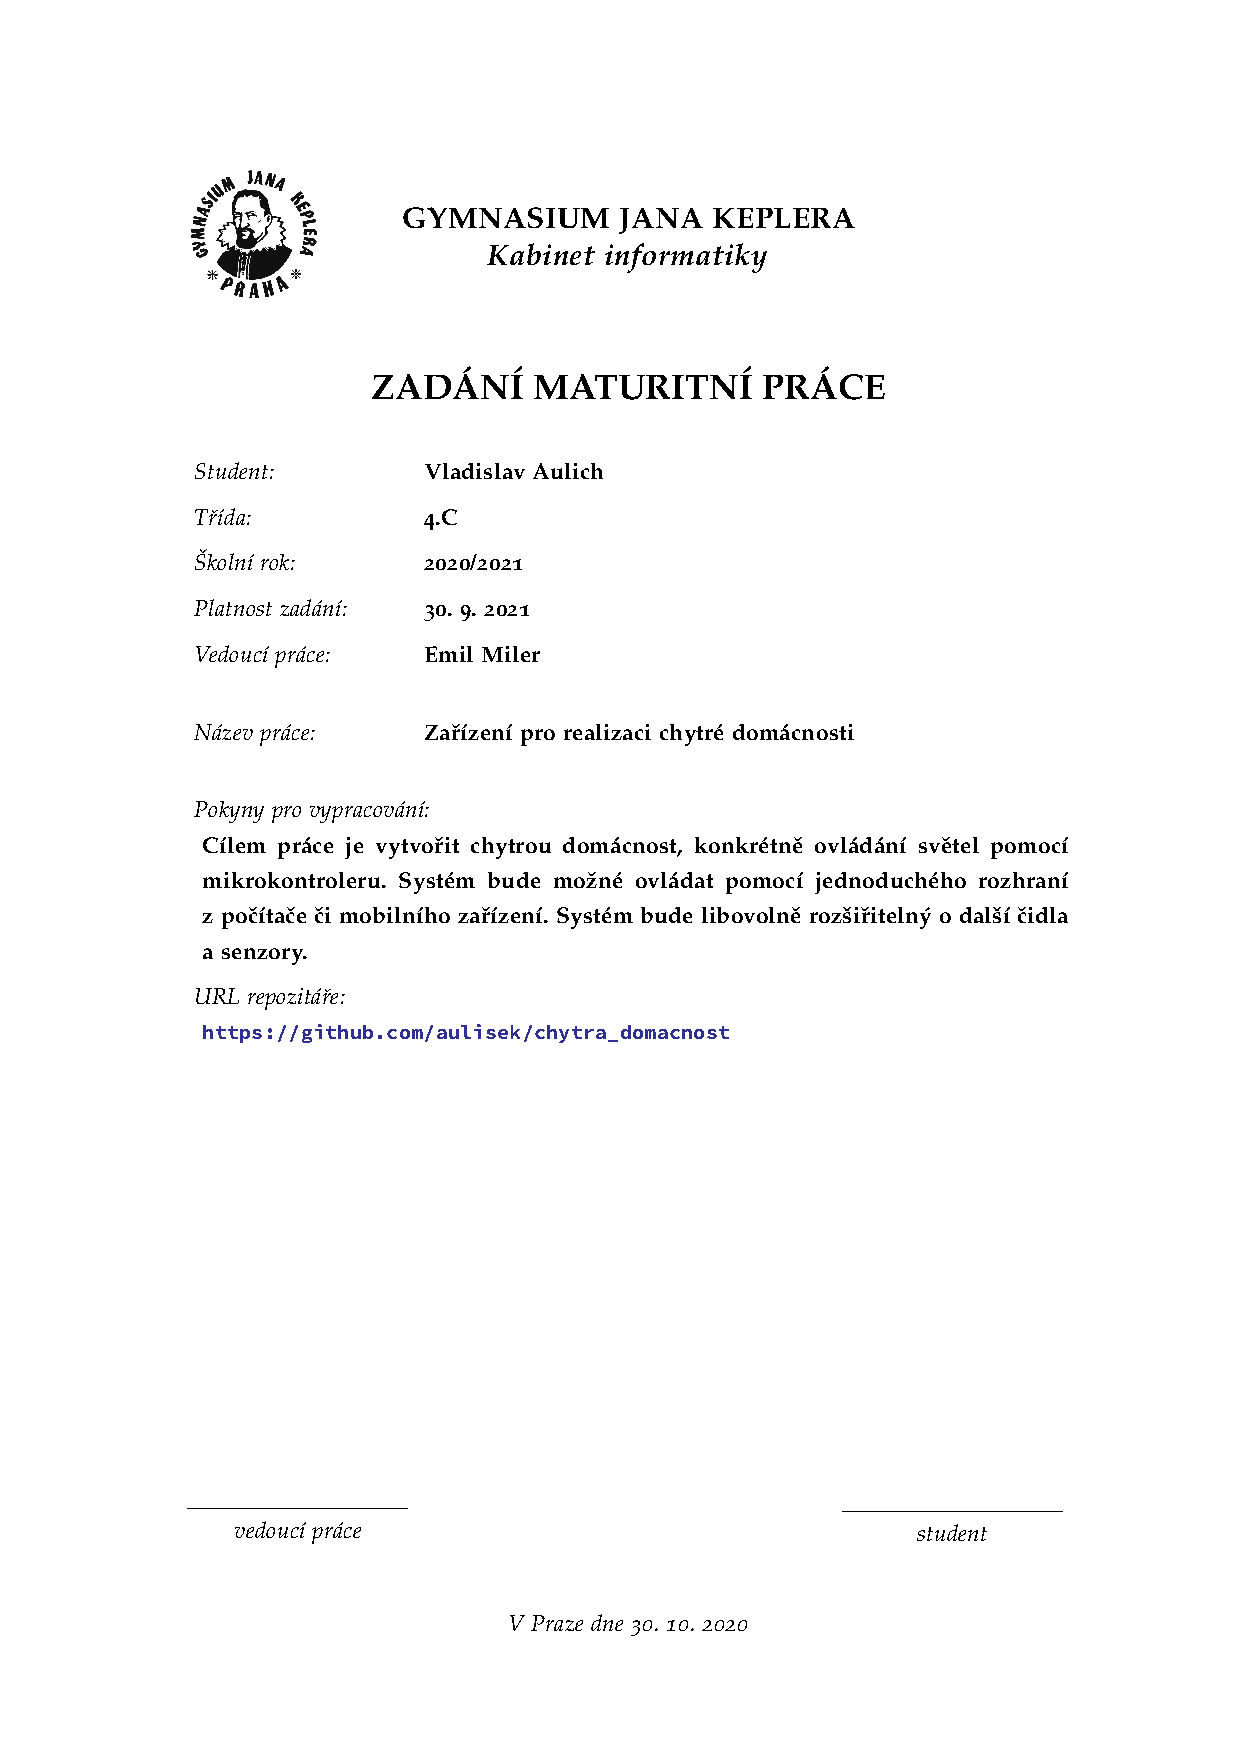
\includepdf[]{zadani.pdf}


%%% Strana s čestným prohlášením k bakalářské práci

\hypersetup{pageanchor=true}
\cleardoublepage
\vspace*{\fill}
\section*{Prohlášení}
\noindent
\Prohlaseni

\vspace{2cm}
\noindent
V Praze dne \today
\hspace*{\fill}\small{\AutorPrace}
\vspace{1cm}

%%% Poděkování
\openright
\vspace*{\fill}
\section*{Poděkování}
\noindent
\Podekovani
\vspace{1cm}


%%% Povinná informační strana bakalářské práce
\openright
\section*{Abstrakt}
\noindent
\Abstrakt
\subsection*{Klíčová slova}
\noindent
\KlicovaSlova

\bigskip\bigskip\bigskip
\section*{Abstract}
\noindent
\AbstraktEN
\subsection*{Keywords}
\noindent
\KlicovaSlovaEN

\openright
\pagenumbering{arabic}

% Obsah
\setcounter{tocdepth}{2}
\tableofcontents

\chapter{Teoretická část}
\pagestyle{fancy}

V první části maturitní práce by se měla objevit informace o tom, jaký problém řešíte. Co si Váš projekt klade za cíl?

\section{Úvod}

Toto téma jsem si zvolil, protože jsem chtěl blíže prozkoumat práci s platformou Arduino a ESP32. S programováním těchto zařízení jsem měl minimální zkušenosti, proto pro mě byla práce na projektu výzvou k objevování nového. Použití komunikace na rádiové frekvenci jsem zvolil z důvodu široké škály použití a velkého množství příkladů. Zároveň jsem měl doma nevyužívaný ovladač pracující s touto frekvencí.



Motivací k výběru tématu \uv{chytré domácnosti} mi bylo její čím dál větší nasazování v domácnostech a snaha vytvořit si ji po svém. Na mnohých komerčních řešeních mi totiž nevyhovoval způsob ovládání, stejně jako velký zásah do soukromí uživatelů.


\section{Cíl práce}

Cílem této práce je vytvořit zařízení pro realizaci chytré domácnosti. Zařízení si klade za cíl ovládat spotřebiče uživatele na tzv. \uv{na dálku}. Součástí řešení musí být uživatelské rozhraní, možnost další automatizace a možnost ovládání \uv{offline}.


\chapter{Implementace}

Druhá kapitola obsahuje detailní informace o tom, jak probíhala implementace. Zde se objeví zdůvodnění výběru technologií, řešení problémů, na které jste narazili, informace o použitých knihovnách apod. Pochvalte se, nikdo to za Vás neudělá. Přiznejte chyby, není to ostuda.


\section{Schéma řešení}

Pro dosažení cíle práce jsem projekt rozdělil na dvě nezávislá zařízení:

\begin{itemize}
	\item Centrály - brány ovládající další zařízení
	\item Koncového zařízení ovládajícího spotřebič
\end{itemize}

Pro každé zařízení jsem pak implementoval potřebné funkce. Dále bylo potřeba zajistit jejich vzájemnou komunikaci.

\subsection{Centrála}

Pro \uv{centrálu} jsem  si vybral platformu ESP32 a to hned z několika důvodů. Čip má integrovanou wifi, k dispozici je velké množství dokumentace, hardwaru s příklady a knihovnami. Další výhodou je velká komunita, což může pomoct při řešení problémů. Čip lze také integrovat do prostředí Arduino IDE, což umožňuje snadnější práci při tvorbě kódu.


Při výběru jsem zvažoval i platformu raspberry pi, ale odradila mě přítomnost operačního systému, který je zbytečný pro tak malý projekt a velké pořizovací náklady oproti ESP32.

Centrála zajišťuje několik funkcí:
\begin{itemize}
	\item Komunikace s uživatelem
	\item Komunikace mezi zařízeními
	\item Správa uložených zařízení
\end{itemize}

\subsubsection{Komunikace s uživatelem}

Pro komunikaci s uživatelem je vytvořeno jednoduché webové rozhraní umožňující dynamicky vypsat uložená zařízení a přidat nové. Pro tvorbu webového rozhraní jsem zvolil knihovnu ESPAsyncWebServer\footnote{https://github.com/me-no-dev/ESPAsyncWebServer}. Tato knihovna má dobře zpracovanou dokumentaci a pro nasazení v projektu se hodí svými funkcemi. Samotné připojení čipu k Wi-Fi je realizováno pomocí knihovny WiFi\footnote{https://github.com/arduino-libraries/WiFi}.


První verze kódu měly implementovaný jednoduchý synchronní webserver pomocí knihovny WiFi, obsažené v základní verzi Arduina IDE. Toto řešení nebylo vhodné, protože numožňovalo připojení více uživatelů k rozhraní naráz.


Další implementovanou funkcí byla autentifikace uživatele. Tato funkce je zajištěná při odesílání requstu pomocí knihovny ESPAsyncWebServer.


Pro zjednodušení přístupu k uživatelskému rozhraní je na zařízení spuštěn mDNS server na adrese http://esp32.local. Tato funkce je realizována pomocí knihovny ESPmDNS \footnote{https://github.com/espressif/arduino-esp32/tree/master/libraries/ESPmDNS}.


Uživatelské rozhraní je vytvořeno pomocí HTML. HTML soubor je uložen ve vnitřní flash paměti čipu ESP. K ovládání filesystému SPIF je užito knihovny SPIFFS\footnote{https://github.com/espressif/arduino-esp32/tree/master/libraries/SPIFFS}. Tato knihovna obsahuje všechny potřebné funkce.


Pro přidání nového zařízení má uživatel na výběr mezi přidáním koupeného komerčního zařízení nebo přidáním zařízení vyrobeného v rámci tohoto projektu. Postup při zadávání nového zařízení je nastíněn we webovém rozhraní.


Komunikace programu a webového rozhraní je zajištěna pomocí HTTP GET requestů, které program zpracuje a provede potřebné akce. 


\subsubsection{Komunikace mezi zařízeními}

Komunikace mezi zařízeními je realizovaná bezdrátově po frekvenci 433 MHz. Tento druh jsem zvolil z důvodu rozšířenosti a nízkých pořizovacích nákladů modulů. Další nespornou výhodou je dosah, který v optimálním prostředí může být až 200 m.


Další ze zvažovaných řešení byla realizace pomocí Wi-Fi nebo GSM modulu. V prvním případě jsem jako nevýhodu viděl dosah (závislost na dostupnosti připojení). Dále by nebylo tak snadné ovládat zařízení pomocí ovladače. V druhém případě byla nevýhoda cena a potřeba realizace připojení pomocí telefoního operátora.


Ovládání modulů jsem chtěl realizovat pomocí jednoduché knihovny VirtualWire, ale zjistil jsem, že není funkční na čipech ESP. K ovládání jsem tak použil knihovnu RadioHead. 


Pro ovládání \uv{Koncového zařízení} je vyslána zpráva obsahující ID zařízení a tag ON nebo OFF, \uv{koncové zařízení} následně odchytí ID a provede příkaz. Tento systém je do budoucna rozšiřitelný o další tagy pro zařízení, které potřebují k ovlání více příkazů než ON nebo OFF.


Tento navržený systém jsem implementoval, nicméně jsem narazil na problém s ovládáním pomocí komerčního ovladače. K tomuto účelu jsem začlenil knihovnu RCswitch\footnote{https://github.com/sui77/rc-switch}, která umožňuje zobrazit protokol, na jehož základě zařízení komunikují. Poté dokáže vysílat tímto protokolem. 


Ve svém řešení jsem chtěl použít knihovny obě a rozdělit tak ovládání na dvě části, podle toho, jakým způsobem mají komunikovat. Při realizaci tohoto jsem však narazil na problém, že není možné bezdrátový vysílač ovládat dvěma knihovnami současně.


Nakonec jsem vybral knihovnu RCswitch z důvodu větší spolehlivosti při přenosu vysílání a možného rozšíření na ovládání komerčních zařízení (nebo ovládání komerčními zařízeními). Toto řešení sebou nese nutnost dvou kódů, pro zapnutí a vypnutí.


\subsubsection{Správa uložených zařízení}

Zařízení se ukládají přímo do flash paměti ESP32 o velikosti 4 MB. Soubor je nazván \uv{zarizeni.csv}.


Do sloupce \uv{název} se uloží název, který si zadá sám uživatel v uživatelském rozhraní. Do sloupce \uv{kod\_ovladac} se v případě zařízení vyrobeného v rámci projektu uloží \uv{x}, protože k ovládání stačí ID zařízení, které je v tomto případě ve sloupci \uv{kod\_zarizeni}.


Při zadávání komerčního zařízení záleží na způsobu ovládání daného zařízení. Při tvorbě jsem vycházel z mého ovladače, který má zvlášť kód pro vypnutí a zapnutí. Jiná zařízení mají odlišná schémata. 


Pro implementaci takového typu zařízení je za potřebí analyzovat, jaký způsob ovládání zařízení používá. K tomu slouží example kód knihovny, který jsem nahrál na jedno ze svých zařízení. Pro funkčnost ovládání je také potřeba prostudovat dokumentaci k této knihovně a dopsat správný typ ovládání do místa v kódu (Toto místo je označeno přímo v kódu).

\subsection{Koncové zařízení}

Toto je hlavní částí mého projektu. Koncové zařízení provádí následující funkce:

\begin{itemize}
	\item přijímá požadavek od centrály
	\item zapne/vypne spotřebič
	\item reaguje na pohyb
	\item obsahuje senzor světla 
	\item reaguje na vstup uživatele z tlačítka
\end{itemize}

Pro \uv{koncová zařízení} jsem zvolil jako vývojovou platformu Arduino uno. Po odladění kódu a hardwaru jsem vyrobil prototyp, který již využíval Arduino Pro mini. 


Pro realizaci zapínání a vypínání spotřebičů jsem zvolil ovládání pomocí relé. Pro snadnější ovládání jsem vybral již hotový modul pro arduino\footnote{https://dratek.cz/arduino/2954-modul-rele-5v-1-kanal-opticky-oddeleno.html}, který pokud je na vstupu logická 1 vypnutý, pokud je přítomna zem, tak je zapnutý (je tzv. negovaný).


Reakce na pohyb je zajišťována PIR senzorem. Opět byl zakoupen modul, který bylo snazší implementovat. Aby nedocházelo k zapnutí světla ve dne, byl k senzoru přidán fotorezistor, který reaguje na hladinu světla v místnosti.


\subsubsection{Tvorba prototypu}



\section{Kalkulace nákladů}
\begin{tabular}{|c|c|c|}
	\hline
	Počet kusů & Název & Cena [Kč] \\
	\hline
	1 & NodeMCU-32S ESP32 & 249  \\
	\hline
	2 & 433 MHz vysílač a přijímač & 79 \\
	\hline
	2 & Spirálová anténa 433 MHz & 10 \\
	\hline
	1 & Mikrospínač & 4 \\
	\hline
	2 & Relé modul s optickým oddělením & 65 \\
	\hline
	1 & Rezistor 10k & 1 \\
	\hline
	1 & Arduino Pro Mini & 98 \\
	\hline
	1 & Arduino uno & 599 \\
	\hline
	1 & PCB prototypová deska & 18 \\
	\hline
	1 & PIR detektro pohybu & 38 \\
	\hline
\end{tabular}

Celkové náklady na \uv{centrálu} jsou přibližně 290 Kč.
Celkové náklady za prototyp \uv{koncového zařízení} jsou 265 Kč.
\chapter{Technická dokumentace}

Poslední kapitola obsahuje informace o tom, jak projekt, který v rámci maturitní práce vznikl, nainstalovat, spustit a používat.

\section{Ukázka sekce}


\subsection{A jedné podsekce}


\section{A další sekce}


\chapter*{Závěr}
\pagestyle{empty}
\addcontentsline{toc}{chapter}{Závěr}

Závěr obsahuje shrnutí práce a vyjadřuje se k míře splnění jejího zadání. Dále by se zde mělo objevit sebehodnocení studenta a informace o tom, co nového se naučil a jak vnímal svou práci na projektu.

%%% Seznam použité literatury
\nocite{einstein}\nocite{latexcompanion}\nocite{knuthwebsite}
\printbibliography[title={Seznam použité literatury},heading={bibintoc}]

%%% Seznam obrázků
\openright
\listoffigures
\addcontentsline{toc}{chapter}{Seznam obrázků}

%%% Seznam tabulek
\clearpage
\listoftables
\addcontentsline{toc}{chapter}{Seznam tabulek}

%%% Přílohy k práci, existují-li. Každá příloha musí být alespoň jednou
%%% odkazována z vlastního textu práce. Přílohy se číslují.

%\part*{Přílohy}
%\appendix

\end{document}
